\documentclass{article}
\usepackage[utf8]{inputenc}

\usepackage{amsmath,amssymb}
\usepackage{mathtools}
\usepackage{xspace}
\usepackage{booktabs}
\usepackage{xcolor}
\usepackage{colortbl}
\usepackage{multirow}
\usepackage{array}
\usepackage{hyperref}
\usepackage{url}
\usepackage{makecell}
\usepackage{changepage}
\usepackage{changes}
\renewcommand\UrlFont{\color{blue}\rmfamily}

\usepackage{float}
\usepackage{booktabs}
\usepackage{longtable}
\usepackage{nicefrac}
\usepackage{amssymb}
\usepackage{amsmath}
\usepackage{xspace}
\usepackage{mathtools}
\usepackage{diagbox}
\usepackage{graphics}
\usepackage{rotating}
\usepackage[algo2e,ruled,vlined,linesnumbered]{algorithm2e}
\newcommand{\assign}{\leftarrow}
\usepackage{graphicx}
\usepackage{subfigure}
\usepackage{ifthen}
\usepackage{wrapfig}
\usepackage{balance} 
\usepackage{epsfig}
\usepackage{xcolor, colortbl}
\usepackage[normalem]{ulem}
\usepackage{dsfont}
\usepackage[algo2e,ruled,vlined,linesnumbered]{algorithm2e}
\usepackage{url}

\graphicspath{ {./images/} }

\newcommand{\tool}{\textsc{{IOHprofiler}}\xspace}
\newcommand{\ioh}{iterative optimization heuristic\xspace}

\newcommand{\oea}{$(1 + 1)$~EA\xspace}
\newcommand{\oeamu}{$(1 + 1)$~EA$_\mu$\xspace}
\newcommand{\ooea}{\oea}
\newcommand{\opl}{$(1+\lambda)$~EA\xspace}
\newcommand{\mpoea}{$(\mu+1)$~EA\xspace}
\newcommand{\opll}{$(1+(\lambda,\lambda))$~GA\xspace}
\DeclarePairedDelimiter{\nint}\lfloor\rfloor


\newcommand{\moga}{$(\mu +1)$~GA\xspace}
\newcommand{\irace}{\textsc{irace}\xspace}
\newcommand{\smac}{\textsc{SMAC}\xspace}
\newcommand{\mlga}{$(\mu+\lambda)$~GA\xspace}
\newcommand{\mhalf}{$(\mu+\mu/2)$~GA\xspace}

\DeclareMathOperator{\select}{select}
\DeclareMathOperator{\SBM}{SBM}
\DeclareMathOperator{\flip}{flip}
\DeclareMathOperator{\opt}{opt}

\newcommand{\LO}{\textsc{LO}\xspace}

\newcommand{\nguyen}[1]{\textbf{\textcolor{blue}{Nguyen: #1}}}
\newcommand{\carola}[1]{\textbf{\textcolor{red}{Carola: #1}}}
\newcommand{\andre}[1]{\textbf{\textcolor{cyan}{Andre: #1}}}

\newcommand{\R}{\mathbb{R}}
\newcommand{\N}{\mathbb{N}}

\title{Dynamic Algorithm Configuration for \opll via irace/SMAC}
% \author{Nguyen, Andre, Carola, Maxim, Roman}
% \date{June 2021}

\begin{document}

\maketitle

\section{Background}

This is an intern project with Deyao Chen (dc262@st-andrews.ac.uk) at the University of St Andrews. In this project, we look into using an automated algorithm configurator to search for the best dynamic policy for $\lambda$ in the \opll (Algorithm~\ref{alg:onell}).

\begin{algorithm2e}[!h]%
\textbf{Initialization:} 
		Sample $x \in \{0,1\}^n$ u.a.r.\;
\textbf{Optimization:}
\For{$t=1,2,3,\ldots$}{
%%%%
    $\lambda \leftarrow p(f(x))$ \\
    \underline{\textbf{Mutation phase:}}\\
    \Indp
    	Sample $\ell$ from $Bin_{>0}(n,p=\lambda/n)$\;
    	\lFor{$i=1, \ldots, \nint{\lambda}$}{$x^{(i)} \assign mutation_{\ell}(x)$}
    	Choose $x' \in \{x^{(1)}, \ldots, x^{(\lambda)}\}$ with $f(x')=\max\{f(x^{(1)}), \ldots, f(x^{(\lambda_1)})\}$ u.a.r.\;
    \Indm
\underline{\textbf{Crossover phase:}}\\
\Indp
\lFor{$i=1, \ldots, \nint{\lambda}$}{$y^{(i)} \assign crossover_{c=\lambda}(x,x')$}
Choose $y \in \{x',y^{(1)}, \ldots, y^{(\lambda)}\}$ with $f(y)=\max\{f(x'),f(y^{(1)}), \ldots, f(y^{(\lambda)})\}$ u.a.r.\;
\Indm
\underline{\textbf{Selection and update step:}}\\
\Indp
\lIf{$f(y)>f(x)$}{
$x \assign y$; }
\Indm
}
\caption{The \opll algorithm with one dynamic parameter to be controlled ($\lambda$). Input is a policy $p$ that maps each $f(x)$ value to the corresponding $\lambda$.}
\label{alg:onell}
\end{algorithm2e}


\section{Experiments}

\subsection{Experiment setting}
We consider 5 problem sizes: $n \in \{50,100,200,500,1000\}$ and two tuning settings:
\begin{itemize}
    \item static-$\lambda$: $\lambda$ is fixed for the whole run of \opll. The tuning budget for this is 1 million or $n$ (the length of the bit string) multipied by $10000$, whichever is smaller.
    \item dynamic-$\lambda$: we search for a policy $p$ that maps each $f(x)$ to a specific $\lambda$. In other words, the number of parameters to be tuned is equal to the problem size $n$. Tuning budget for this setting is $n$ (the length of the big string) multiplied by 100.
\end{itemize}

The following baselines are used for the comparisons:
\begin{itemize}
    \item Five Parameters: the 5-parameter dynamic \opll with the best parameter setting found by \irace in our GECCO2019 paper.
    \item Dynamic Theory: $\lambda$ is controlled by the one-fifth success rule.
    \item $\lambda=1$ for the whole run.
    \item Random $\lambda$: using a randomly generated policy $p$ for every run.
\end{itemize}

\subsection{Results with \irace}

\begin{figure}[ht]
    \centering
        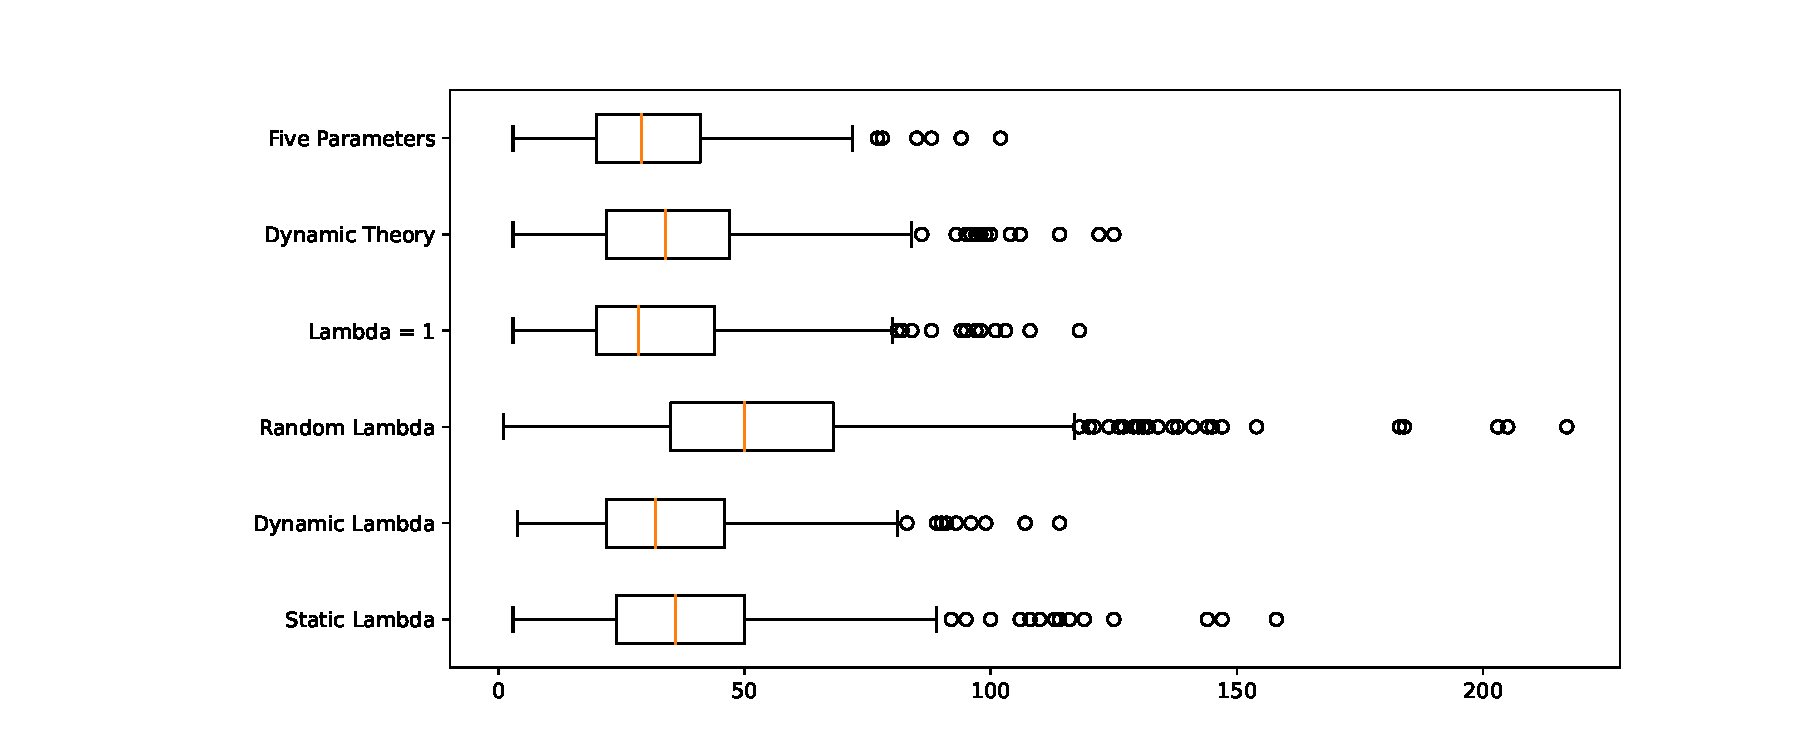
\includegraphics[width=1.0\textwidth]{box_plot_10_100_10000.pdf}
        \caption{The performance comparison for $n = 10$ and a tuning budget of $100000$ for dynamic-$\lambda$ and $1000$ for static-$\lambda$}
        \label{box_plot_10_100_10000}
\end{figure}

\begin{figure}[ht]
    \centering
        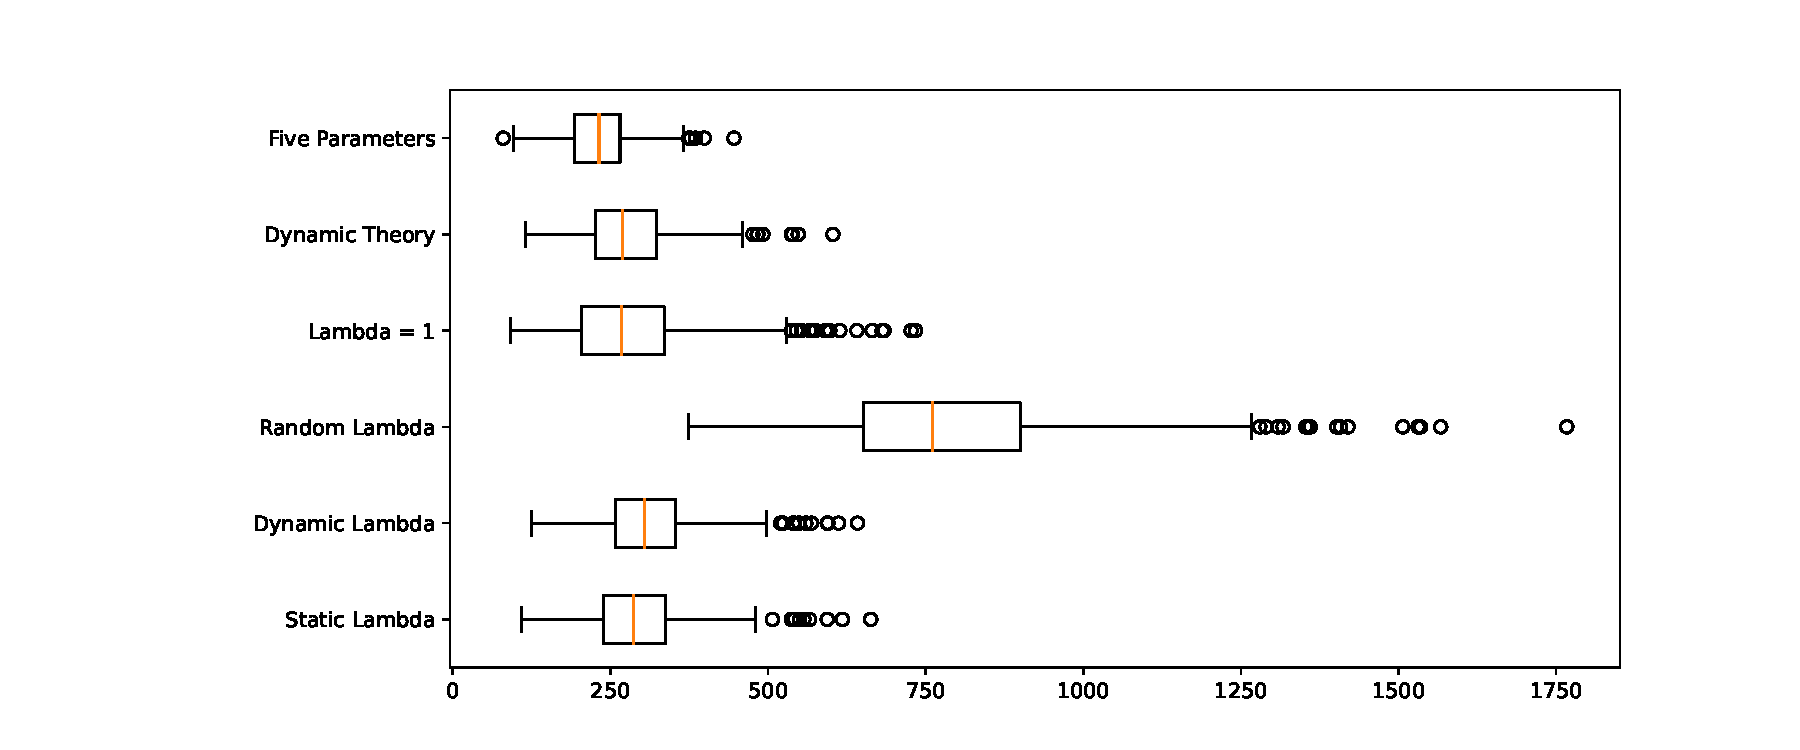
\includegraphics[width=1.0\textwidth]{box_plot_50_100_10000.pdf}
        \caption{The performance comparison for $n = 50$ and a tuning budget of $500000$ for dynamic-$\lambda$ and $5000$ for static-$\lambda$}
        \label{box_plot_50_100_10000}
\end{figure}

\begin{figure}[ht]
    \centering
        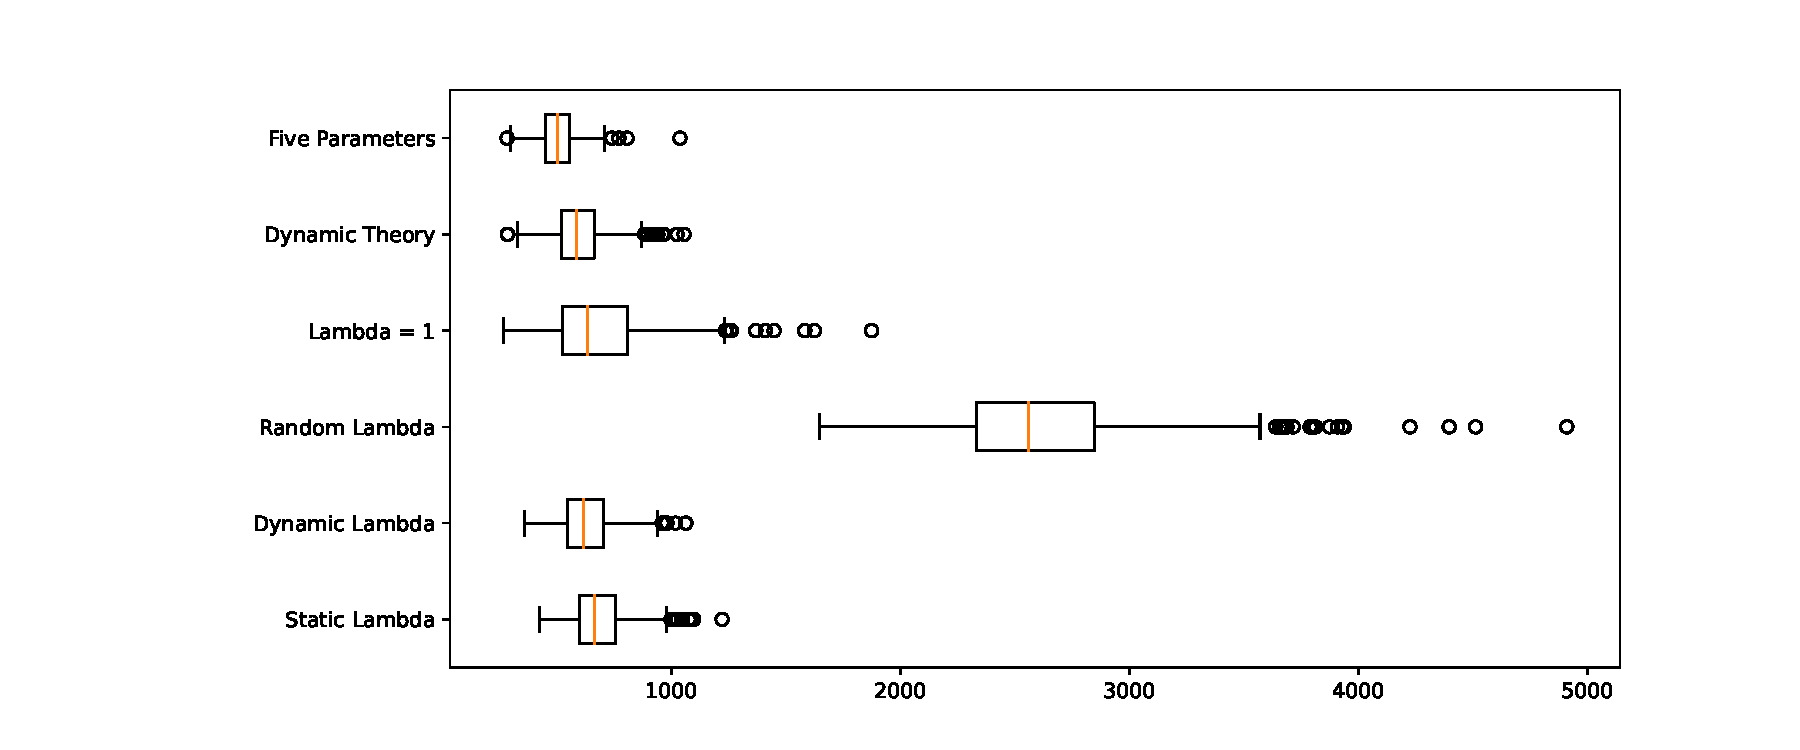
\includegraphics[width=1.0\textwidth]{box_plot_100_100_10000.pdf}
        \caption{The performance comparison for $n = 100$ and a tuning budget of $1000000$ for dynamic-$\lambda$ and $10000$ for static-$\lambda$}
        \label{box_plot_100_100_10000}
\end{figure}

\begin{figure}[ht]
    \centering
        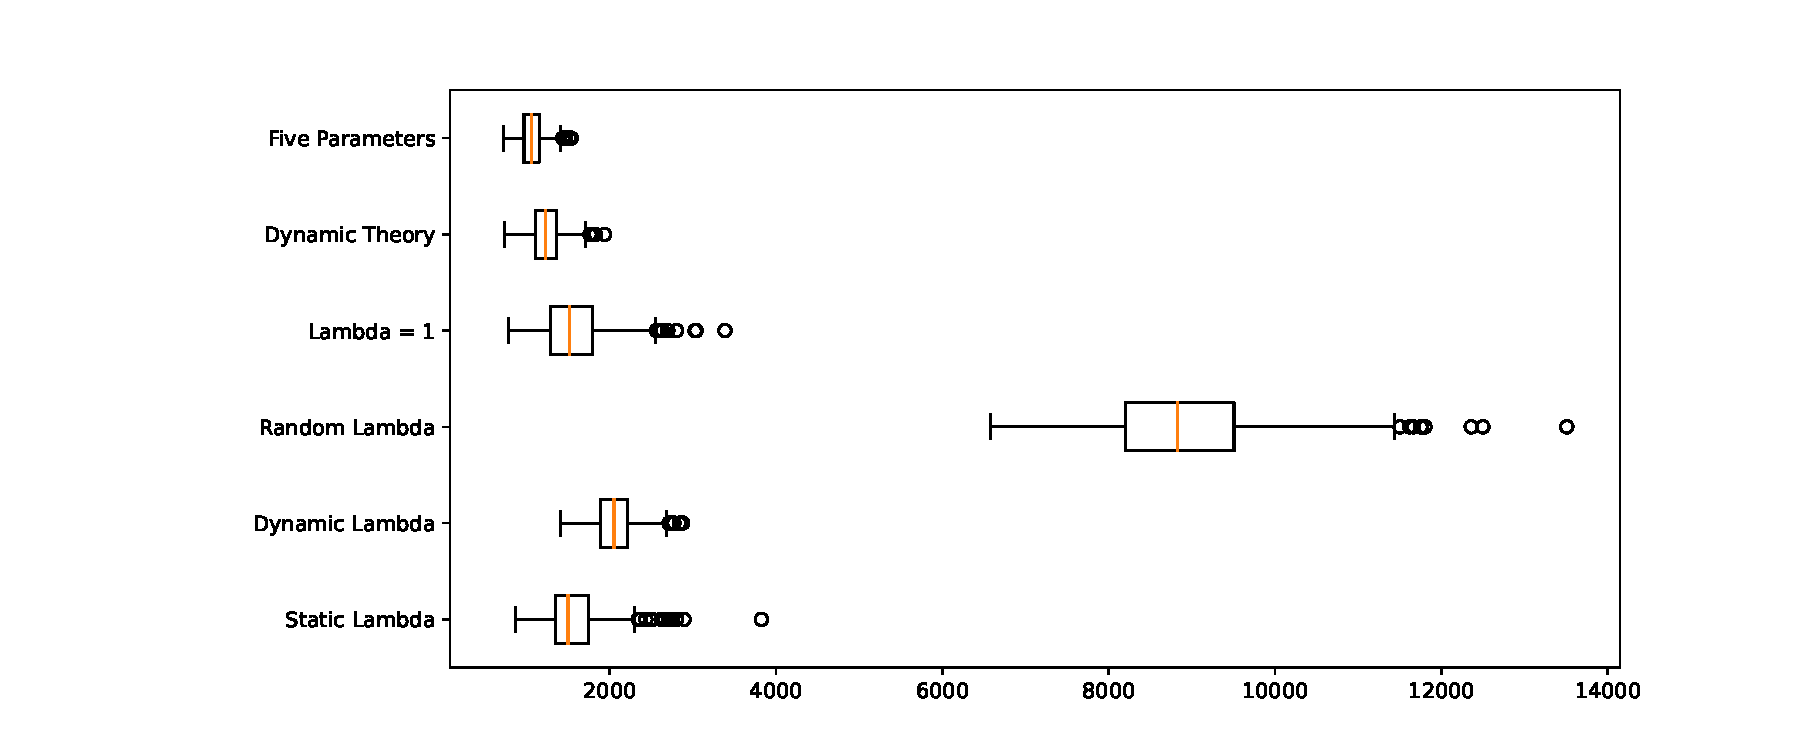
\includegraphics[width=1.0\textwidth]{box_plot_200_100_5000.pdf}
        \caption{The performance comparison for $n = 200$ and a tuning budget of $1000000$ for dynamic-$\lambda$ and $20000$ for static-$\lambda$}
        \label{box_plot_200_100_5000}
\end{figure}

\begin{figure}[ht]
    \centering
        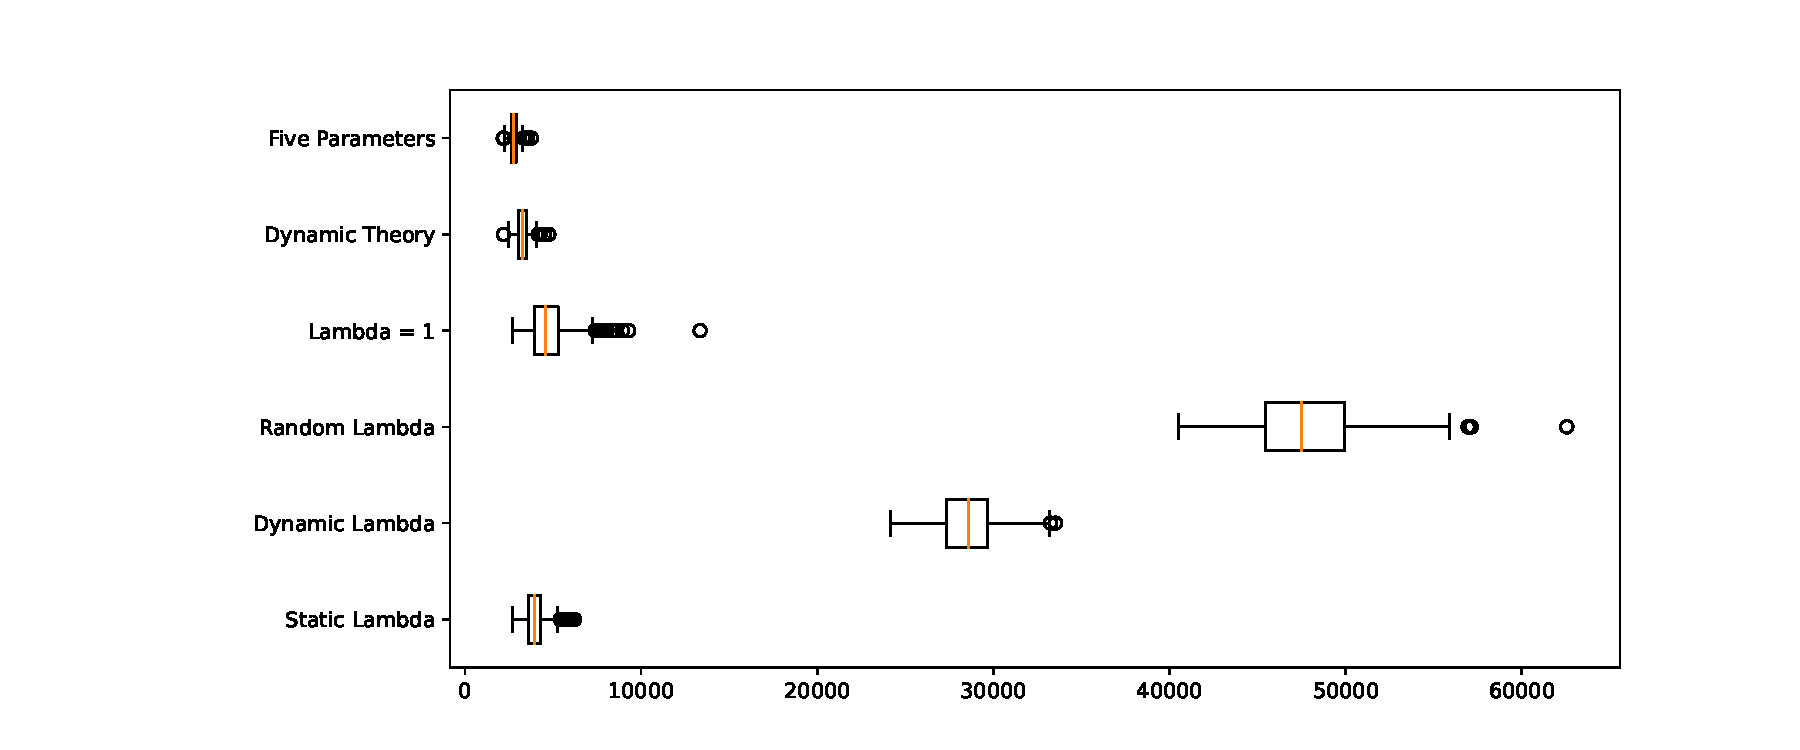
\includegraphics[width=1.0\textwidth]{box_plot_500_100_2000.pdf}
        \caption{The performance comparison for $n = 500$ and a tuning budget of $1000000$ for dynamic-$\lambda$ and $50000$ for static-$\lambda$}
        \label{box_plot_500_100_2000}
\end{figure}

\begin{figure}[ht]
    \centering
        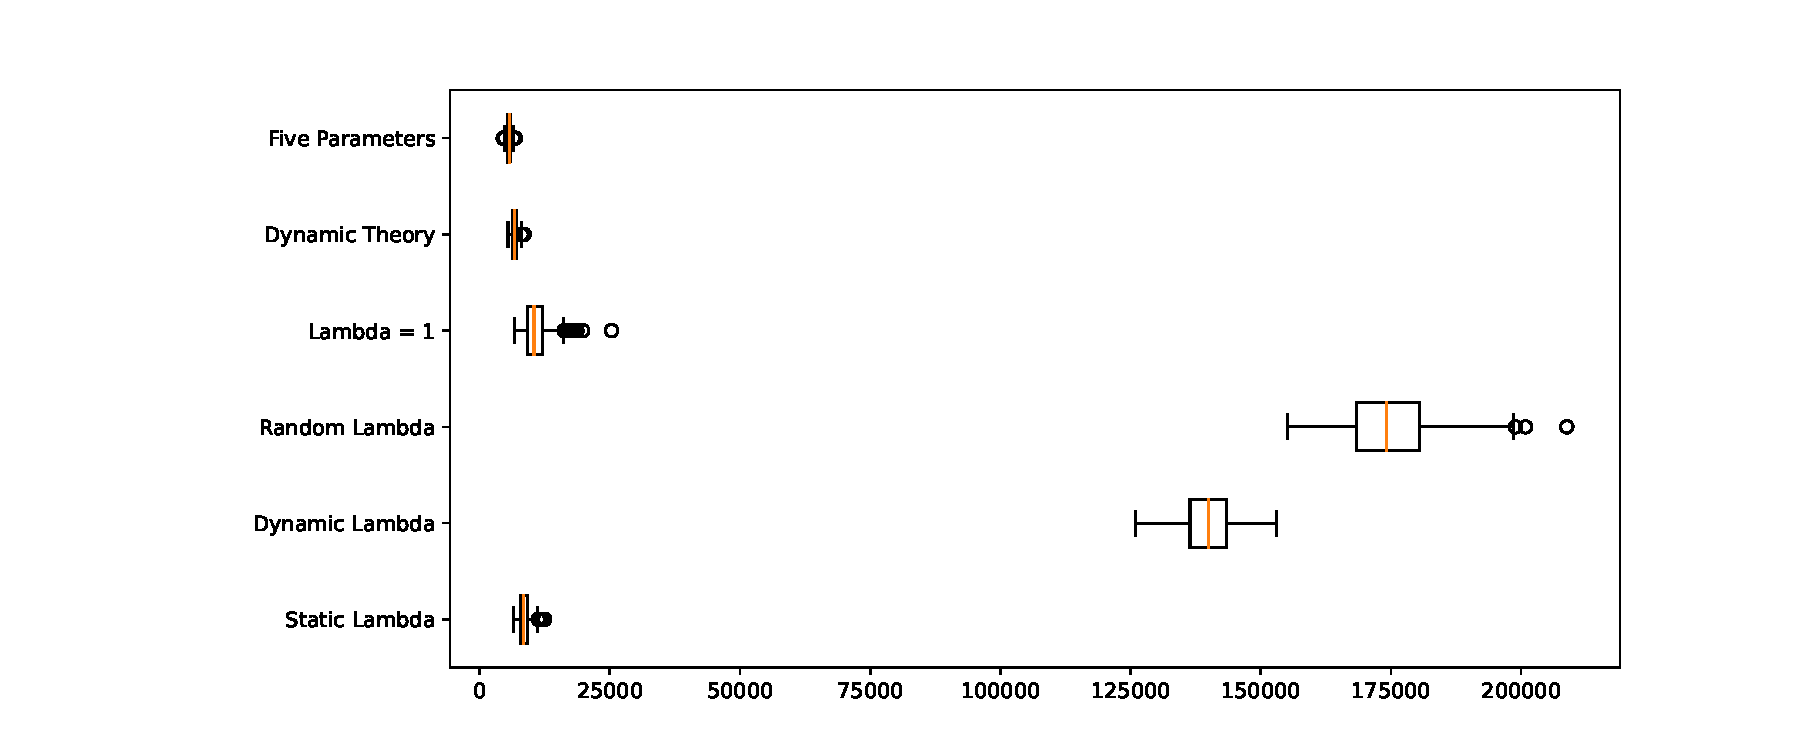
\includegraphics[width=1.0\textwidth]{box_plot_1000_100_1000.pdf}
        \caption{The performance comparison for $n = 1000$ and a tuning budget of $1000000$ for dynamic-$\lambda$ and $100000$ for static-$\lambda$}
        \label{box_plot_1000_100_1000}
\end{figure}

\subsection{Results with \smac}

\end{document}
